\section{Experiments and Results - Need to add comparison to Song and Set cover}

\subsection{Reference algorithms}
The implementation was done using Spark~\cite{spark}. As the baseline, Spark mlib has an implementation of PFP (Add link to github?). For our experiments, we leveraged that implementation and the edits required for IPFIM where minor:
\begin{steps}
\item Added support for 
\end{steps}
For CanTree experiments, as can be seen From [link to IPFIM algorithm], running IPFIM with numGroups = 1, will result in CanTree algorithm.

For the algorithm developed in Song, we had to add a functionality to

The used hardware is 4 clusters each with 20G memory and 40 cores. Also used is SparkRDMA Plugin~\cite{SparkRDMA}.  Elaborate in a new section?

\subsection{Datasets}
For this article, we used 2 types of datasets:
\begin{enumerate}
\item Synthetic datasets of 100M, 10M and 1M transactions, and 2 magnitudes less of items, average length of 20 and 15 items. The datasets were generated using IBM Quest Synthetic Data Generator ~\cite{agrawal1994quest}. 
\item The Kosarak dataset contains 990,000 transactions with 41,270 distinct items and an average transaction length of 8.09 items (click-stream data of a hungarian on-line news portal). This dataset was the largest used by ~\cite{tanbeer2009efficient}.
\end{enumerate}


All the test cases were divided in to 50\% base case and the remaining 50\% to iterations of 2.5\% (e.g. 20 iterations).


For PFP~\cite{li2008pfp} performance comparison, Spark~\cite{spark} mllib package implements just that, and was used per iteration.


\subsection{IPFIM vs PFP}
 For correct PFP~\cite{li2008pfp} mining, a read of all the dataset till that point needs to be performed.
\subsubsection{Synthetic Dataset}
A comparison for 10M transactions (T15D10MN100K) with minSupport of 0.001, 1K partitions is seen at \autoref{fig:PFPvsIPFP}.

\subsubsection{Kosarak Dataset}
A comparison with minSupport of 0.001, partitions of 10 and 100 is seen at \autoref{fig:PFPvsIPFPKos}.


\begin{figure}
  \centering
  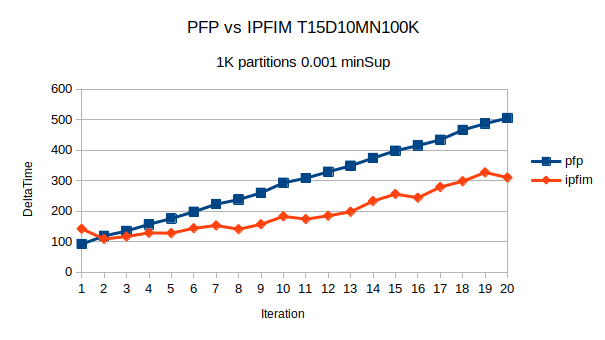
\includegraphics[width=\linewidth]{figures/PFPvsIPFIM0_001_10M}
  \caption{PFP vs IPFIM 10M}
  \label{fig:PFPvsIPFP}
\end{figure}

\begin{figure}
  \centering
  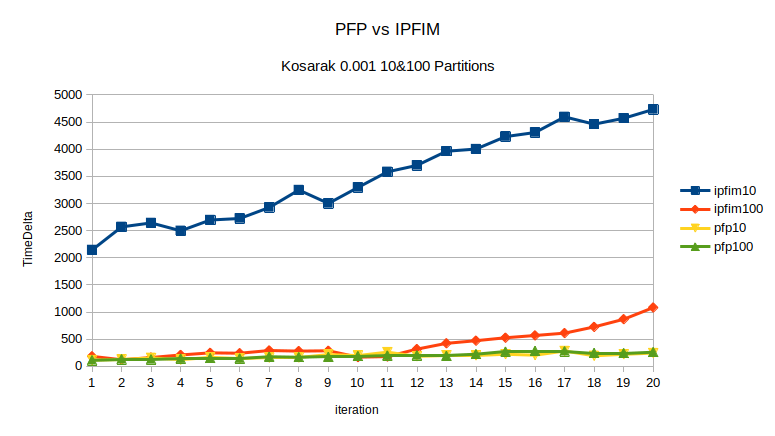
\includegraphics[width=\linewidth]{figures/PFPvsIPFIM0_001_Kosarak}
  \caption{PFP vs IPFIM Kosarak}
  \label{fig:PFPvsIPFPKos}
\end{figure}


\subsection{IPFIM vs CanTree}
For CanTree~\cite{leung2005cantree} performance, we used IPFIM with only one group, meaning a single tree.

\subsubsection{Synthetic Dataset}
A comparison for 1M transactions (T15D1MN10K) with minSupport of 0.001, partitions of 1, 10 and 100 is seen at \autoref{fig:IPFP1M0001}.

\subsubsection{Kosarak Dataset}
A comparison with minSupport of 0.001, partitions of 1, 10 and 100 is seen at \autoref{fig:IPFP1M0001_10_100}.


\begin{figure}
  \centering
  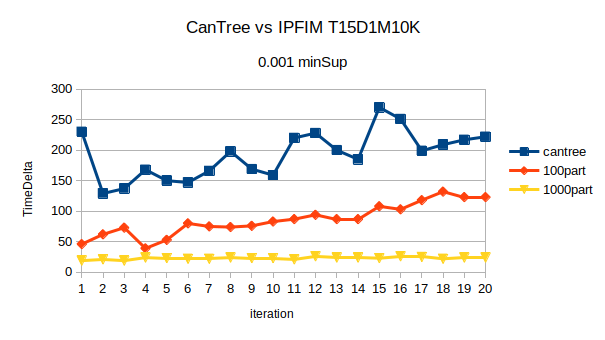
\includegraphics[width=\linewidth]{figures/IPFP1M0001}
  \caption{Inc. vs IPFIM}
  \label{fig:IPFP1M0001}
\end{figure}

\begin{figure}[h!]
  \centering
  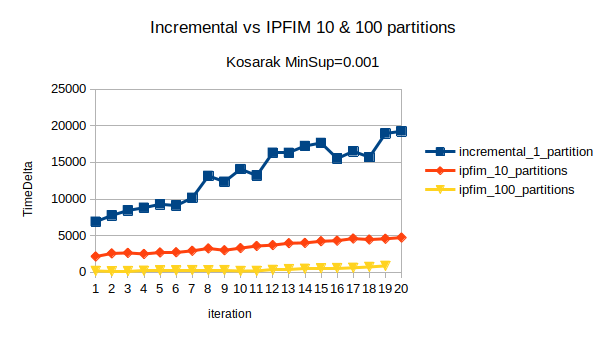
\includegraphics[width=\linewidth]{figures/IPFIM_1_10_100_part_kosarak}
  \caption{Inc. vs IPFIM 10 \& 100 partitions}
  \label{fig:IPFP1M0001_10_100}
\end{figure}

